\documentclass[10pt]{article}
\newcommand{\HRule}{\rule{\linewidth}{0.5mm}}
\parindent 0pt
\parskip 10pt
\usepackage{anysize}
\usepackage{graphicx}
\usepackage{epsfig}
\usepackage{float}
%\usepackage{cite}
\usepackage{natbib}
\usepackage{setspace}
\marginsize{3.5cm}{3.5cm}{1cm}{1cm}
\onehalfspacing
\usepackage{caption}
\usepackage{subcaption}
\usepackage{amsmath,hyperref}

\usepackage{xcolor}
\hypersetup{
    colorlinks,
    linkcolor={red!50!black},
    citecolor={blue!50!black},
    urlcolor={blue!80!black}
}

%\textwidth 15cm
%\textheight 24cm
%\onehalfspacing
\begin{document}

\title{Biomechanical Features of Orthopaedic Patients}

\author{David Starkey}

\maketitle





\section{Introduction and Data Source}



Internet Of Things (IOT) is a machine learning approach to providing smart, inter-connectivity between technologies that exist currently in isolation to perform 'common sense' intuitive tasks. In the context of medical care, IOT has the potential to improve Connected care. Connected care is the real time electronic communication between patient and provider currently applied to areas such as remote patient monitoring and secure email communication between carer and patient. In this project, I analyse a sensor dataset taken of orthopaedic patients to identify the factors that trigger a spinal condition known as Spondylolisthesis. This is the slipping of vertebra that occurs, in most cases, at the base of the spine The problem also involves predicting the grade, class or severity of the condition given a set of input attributes including pelvic incidence, pelvic tilt, lumbar lordosis angle, sacral slope and pelvic radius for around 400 patients. The entire dataset is described and available here \footnote{\href{ https://www.kaggle.com/uciml/biomechanical-features-of-orthopedic-patients}{\textcolor{blue}{https://www.kaggle.com/uciml/biomechanical-features-of-orthopedic-patients}}}. The analysis will use a Classification And Regression Tree (CART) supervised learning approach to determine the most imprtant attributes giving rise to the condition and to classify the patients based on the severity of Spondylolisthesis. The technical algorithmic details of the CART process are detailed in the Section \ref{sec_rf} and results are presented in Section \ref{sec_res}




\section{Random Forest Regression Analysis}
\label{sec_rf}
This section will detail the statistical algorithm used to classify the data for the interested reader. The layperson is welcome to skip to the results section for the summary of the main finding.

The random forest decision tree classifier is a rather complex algorithm with many steps. A disadvantage to this algorithm (as will become apparent after following the steps below) is that it has a large number of tunable `hyper parameters' that must be set for the decision tree to work. While more simple algorithms like $k$ means clustering are very direct with no `tune-ing' requirements, a random forest requires the user to specify the number of trees in the forest, the depth of each tree, the cost function and in some cases the method by which to assign the class (i.e should we average the probability distributions from each tree or use the mode class from each tree to assign the class). Despite this draw back, however, random forest classifiers are very visual classifiers for a general audience to understand intuitively even if the full details of the algorithm are unclear. They are also quite robust and provide very accurate classifications in general. The algorithm for creating a single tree is as follows:

\begin{itemize}
\item Arrange the dataset into a matrix $X(N,M)$ where each of the $N$ rows corresponds to one example in and $M$ dimensional feature space. You may need to apply `one-hot-encoding' to convert categorical variables into a binary matrix format. Also arrange the prediction values (purchase amount) into an array $C(M)$.


\item Consider a random set of $K < M$ dimensions in the parameter space and a random subset of $I<N$ points from the data set. 

\item We now need a value $S$ above and below which to split the $I$ considered points. The value of all $I$ points, in each dimension $k \in K$ are considered in turn as the split point $S$.

\item The Cost function for each branch $l$ following the split is given by
\begin{equation}
C_l = \sum_{j=1}^{N_j} \left( y_j - \langle y \rangle \right)^2,
\end{equation}

\noindent where $\langle y \rangle$ denotes the average purchase amount of all points in this branch. The total cost function is given by summing $C_l$ over each of the two child branches. The choice of split $S$ is given by considering, in turn, each point in the subset of $I$ rows and $K$ dimensions as the split $S$. The value of the data matrix that minimises $C$ is chosen as the split point $S = X(i,k)$.


\item Repeat this for each child of the above node and continue to deepen the tree up to a desired depth (e.g 5 levels). Each time a new node is considered, chose a new random set of $K$ dimensions and $I$ points to consider for the split quantity. The choice of depth is somewhat arbitrary but the node path terminates once the tree has reached a certain depth or if there are no children in the branch following a split (no more data left to populate the branch).

\end{itemize}

The above algorithm generates a single decision tree. The random forest algorithm works by constructing an arbitrary number of trees (e.g 5, 10, 50) and propagating new test data through each tree. Each tree will yield a new posterior probability distribution of Spondylolisthesis classes and the average is used as the output of the random forest. 





\section{Results and Conclusions}
\label{sec_res}
The random forest decision tree classifier is applied to the Spondylolisthesis sensor data using a cross validation approach. Of the original 400 patients in the data set, 25\% are selected to serve as a mock test-sample to serve as a measure of the accuracy of the simulation. A forest of five trees is constructed according to the algorithm in Section \ref{sec_rf} and the random forest, once trained on the mock training set, is used to predict the Spondylolisthesis class of the mock test-data set. An example decision tree is shown in Figure \ref{fig_smalltree} and the result of the fits to the mock test data set is shown in Figure \ref{fig_predict}. Figure \ref{fig_predict} shows that the random forest method accurately estimates the Black Friday spending for a given test data set across all values. The estimated accuracy, calculated from the mean absolute error, is approximately 80.0\%. 

The random forest classifier can also be used to assess the importance of each of the variables in affecting the Spondylolisthesis grade. The fractional importance for the most important variables is show in Figure \ref{fig_import}. It can be seen that the xx has the largest affect on the Spondylolisthesis class. 

We also explore a variety of other classifiers based on algorithms from machine learning including both supervised and unsupervised approaches. The accuracy of these approaches as a function of sample size is plotted in Figure \ref{fig_comp}. We see that the CART classifier appears to be the most accurate for this experiment.



Future regression exercises might improve on this data set and attempt to speed up the fits by utilizing only the attributes contributing most of the fractional importance. Careful ranking of the important features of a data set, as performed in this study, is key to successfully combine IoT with connected care.


\begin{figure}
\begin{center}
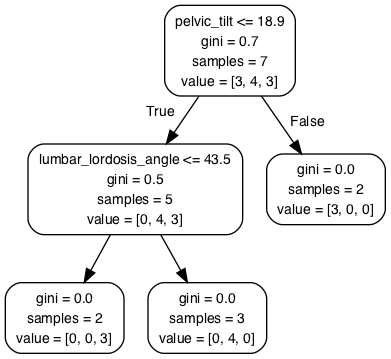
\includegraphics[scale=0.4,angle=0,trim=8cm 0cm 0cm 0cm]{small_tree_0_0.png}
\caption{An example decision tree used to predict the degree of Spondylolisthesis amount. The full tree is much too large to be visualised and so this small example is used as a visual aid.}
\label{fig_smalltree}
\end{center}
\end{figure} 


%\begin{figure}
%\begin{center}
%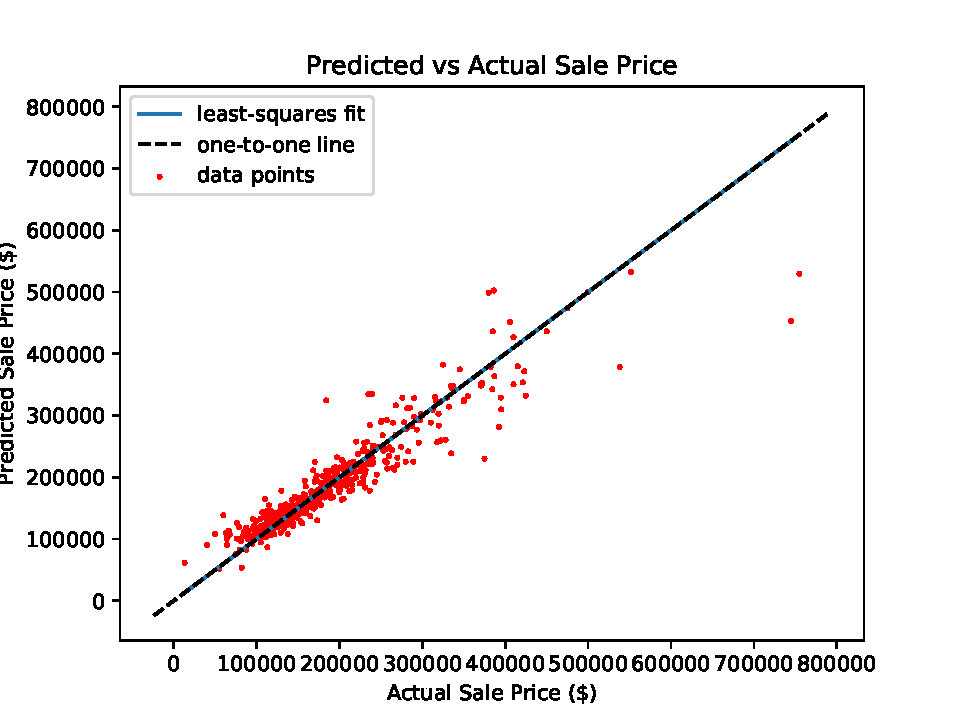
\includegraphics[scale=0.8,angle=0,trim=0cm 0cm 0cm 2cm]{fig_actual_vs_predict.pdf}
%\caption{Actual vs Predicted spend amount after training of the random forest regression algorithm. The dashed line shows the one-to-one correlation line (a 100\% accurate model with no outlying points would show all point lying on this line).}
%\label{fig_predict}
%\end{center}
%\end{figure} 


\begin{figure}
\begin{center}
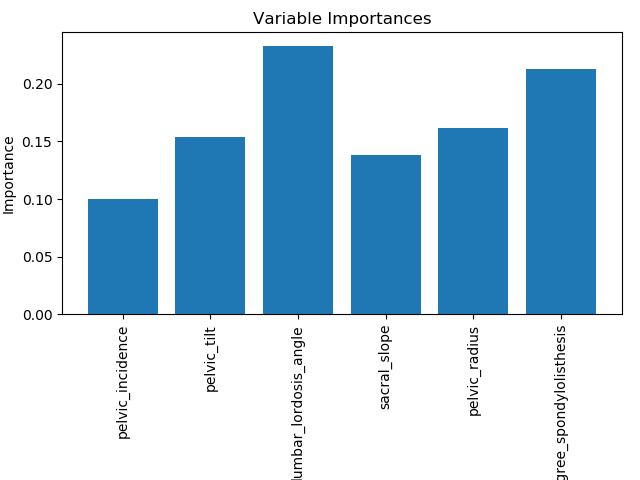
\includegraphics[scale=0.8,angle=0,trim=0cm 0cm 0cm 0cm]{importances_0_0.png}
\caption{Fractional importance of the most important attributes in triggering Spondylolisthesis.}
\label{fig_import}
\end{center}
\end{figure} 



\begin{figure}
\begin{center}
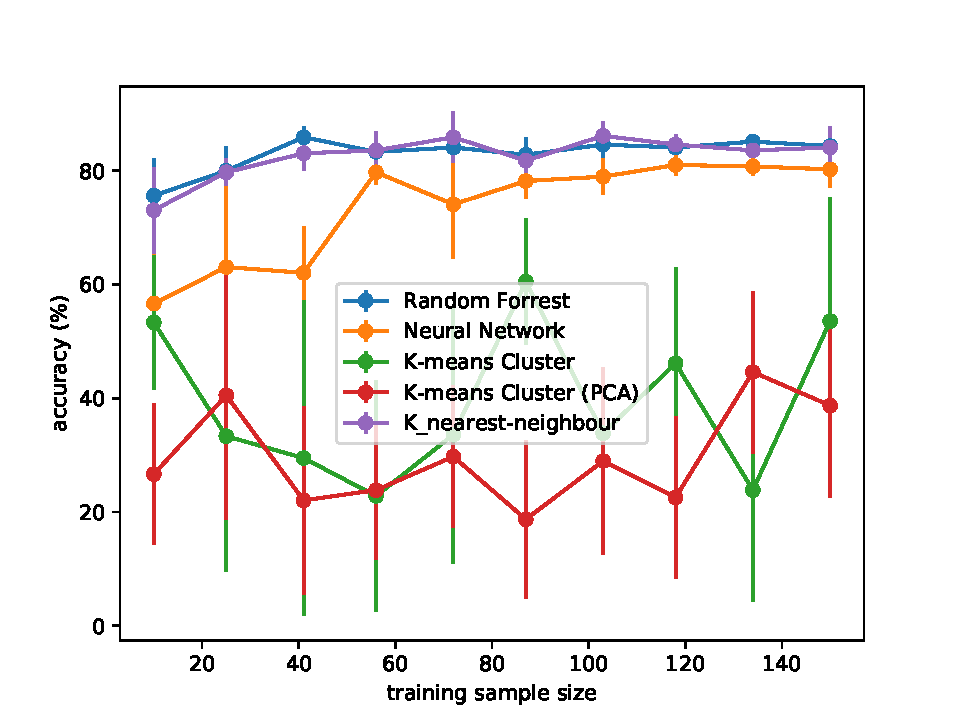
\includegraphics[scale=0.4,angle=0,trim=8cm 0cm 0cm 0cm]{comparison_accuracy.pdf}
\caption{Comparison between CART classifier, multi-layer-neural-net, K-nearest neighbour and K-means classifiers vs sample size.}
\label{fig_comp}
\end{center}
\end{figure} 


\begin{table}
\center
\caption{Fractional importance of each of the attributes in the sensor attributes most correlated with Spondylolisthesis.}
\begin{tabular}{cc}
\hline
Attribute & Fractional importance \\
\hline 
\hline
Lumbar lordosis angle & 0.23 \\
Degree Spondylolisthesis & 0.21 \\
Pelvic radius & 0.16 \\
Pelvic tilt & 0.15 \\
Sacral Slope & 0.13 \\
Pelvic Incidence & 0.10 \\
\hline
\end{tabular}
\label{tab_import}
\end{table}


\end{document}



